\documentclass[letterpaper, 10 pt, conference]{ieeeconf}  % Comment this line out if you need a4paper

%\documentclass[a4paper, 10pt, conference]{ieeeconf}      % Use this line for a4 paper

\IEEEoverridecommandlockouts                              % This command is only needed if 
                                                          % you want to use the \thanks command

\overrideIEEEmargins                                      % Needed to meet printer requirements.

% See the \addtolength command later in the file to balance the column lengths
% on the last page of the document

% The following packages can be found on http:\\www.ctan.org
\usepackage{times}
\usepackage{cite}
\usepackage{graphics} % for pdf, bitmapped graphics files
\usepackage{graphicx}
\usepackage{epsfig} % for postscript graphics files
\usepackage{mathptmx} % assumes new font selection scheme installed
%\usepackage{times} % assumes new font selection scheme installed
\usepackage{amsmath} % assumes amsmath package installed
\usepackage{amsfonts}
\usepackage{amssymb}  % assumes amsmath package installed
\usepackage{bm}
\usepackage{soul}
% \usepackage{todonotes}
\usepackage{url}
\usepackage{multicol}
\usepackage{multirow}
\usepackage[bookmarks=true]{hyperref}
\usepackage{verbatim}
\usepackage{color}
\usepackage{tabularx}
\usepackage{booktabs}
\usepackage{listings}
\usepackage{siunitx}
\usepackage[utf8]{inputenc}
\usepackage{pifont}
\usepackage{csquotes}
\usepackage{mathtools}
\usepackage{breqn}
\usepackage{cancel}
\usepackage{xcolor}
\usepackage{optidef}
\usepackage{cleveref}
\usepackage{setspace}

\newcommand{\cmark}{\ding{51}}%
\newcommand{\xmark}{\ding{55}}%

%\makeatletter
%\def\endthebibliography{%
%  \def\@noitemerr{\@latex@warning{Empty `thebibliography' environment}}%
%  \endlist
%}
%\makeatother

\begin{document}
	
\linespread{0.98}
\setlength{\textfloatsep}{1pt}  % Replace X with the desired length in points
\setlength{\intextsep}{1pt}
\setlength{\abovecaptionskip}{1pt}

\title{\LARGE \bf
Optimal Design of Agile Jumping Maneuvers for a Single Leg System
% heavy-duty 
% Impact-Aware Planning and Control of Agile Jumping Maneuvers: from the Thrust Phase to Landing
%Designing Aerial Maneuvers for Agile Legged Systems via Trajectory Optimization: from take-off to landing
%Design and Control of Jumping Maneuvers via Trajectory Optimization: from the Thrust Phase to Landing
}

\author{$^{1\,-\,2}$, Arturo Laurenzi$^{1}$ $^1$
% , Francesco Ruscelli1^{1}, Luca Rossini$^{1}
\thanks{  Please send correspondence to \tt\scriptsize \{andrea.patrizi\}@iit.it}}
\author{%
  \authorblockN{%
    Andrea Patrizi\authorrefmark{1}\authorrefmark{2},
    Francesco Ruscelli\authorrefmark{1}\authorrefmark{3}, 
    Arturo Laurenzi\authorrefmark{1}\authorrefmark{3},
    and Nikos G. Tsagarakis\authorrefmark{1}
  }
%  \authorblockA{\authorrefmark{1} Humanoid and Human-Centred Mechatronics (HHCM), Istituto Italiano di Tecnologia (IIT), Via San Quirico 19d, 16163 Genova}%
%  \authorblockA{\authorrefmark{2} }
}

% footnotes
\maketitle
\begingroup\renewcommand\thefootnote{\authorrefmark{2}}
\footnotetext{Department of Informatics, Bioengineering, Robotics and Systems Engineering, Università di Genova, Via All'Opera Pia 13, 16145 Genova.}
\endgroup
\begingroup\renewcommand\thefootnote{\authorrefmark{1}}
\footnotetext{Humanoids and Human-Centred Mechatronics (HHCM), Istituto Italiano di Tecnologia (IIT), Via San Quirico 19d, 16163 Genova.}
\endgroup
\begingroup\renewcommand\thefootnote{\authorrefmark{3}}
\footnotetext{The authors contributed equally to the manuscript.}
\endgroup

\setlength{\textfloatsep}{12.0pt plus 8.0pt minus .0pt}

%\begingroup\renewcommand\thefootnote{}
%\footnotetext{\{francesco.ruscelli, arturo.laurenzi,
%enrico.mingo, nikos.tsagarakis\}@iit.it}
%\endgroup
%%%%%%%%%%%%%%%%%%%%%%%%%%%%%%%%%%%%%%%%%%%%%%%%%%%%%%%%%%%%%%%%%%%%%%%%%%%%%%%%
\begin{abstract}
In this work we showcase a comprehensive study, developed around our heavy-duty eletrically-actuated quadruped leg prototype, focusing on the task of jumping. Our study employs a two-stage pipeline for the design and execution of agile and efficient jumping maneuvers.
We combine offline non-linear whole-body Trajectory Optimization (TO)
%, which considers the robot's multi-body dynamics and calibrated actuators models
to formulate and solve two distinct non-linear problems, each tackling different phases and performance aspects of the jumping maneuver. 
The first one jointly addresses the thrust and flight phases and aims at maximizing the achieved jump height, while accounting for several hardware limitations.
The second problem deals with the impact and braking phases 
%and optimizes for a landing configuration and joint-space impedances,
%with the objective of 
minimizing the kinetic energy dissipated at the impact, while maximizing the energy regenerated by the actuators during braking. We 
%explore the driving reasons behind our formulations and approach and 
validate the accuracy of the employed models and the results of the optimizations both in simulation and on the real leg hardware, showing the effectiveness of our approach in maximizing hardware performance and the benefits of exploiting combined impact-energy considerations during the execution of jumping maneuvers.
\end{abstract}

\IEEEpeerreviewmaketitle


%%%%%%%%%%%%%%%%%%%%%%%%%%%%%%%%%%%%%%%%%%%%%%%%%%%%%%%%%%%%%%%%%%%%%%%%%%%%%%%%
\section{Introduction}\label{sec:introduction}

 Legged robots are among the most versatile robotic platforms available. As their natural counterpart, they show great flexibility and are particularly suited for applications where navigation through unstructured environments is required. 

The development of robots capable of fully exploiting the potential of legged morphologies is, however, a non-trivial task, both in terms of design and control. There are several instances of robots that come close to achieving this.
% For instance, in~\cite{agile_bots::hawkes2022engineered} the authors employ the work multiplication principle to design and control a miniature robot capable of exceeding the jumping performance of any biological jumper. 
% A hybrid approach is employed by Ascento~\cite{agile_bots::klemm2019ascento}, which uses wheeled-locomotion for normal navigation and jumping motions generated with a multi-phase heuristic feed-forward controller to overcome challenging obstacles.
The autonomous quadruped ANYmal~\cite{agile_bots::hutter2016anymal} is, for instance, an example of a torque-controllable robot capable of robustly navigating through harsh industrial environments while performing complex locomotion tasks.

The potential of legged robots has begun to show its full realization only in recent years, culminating with the latest Boston Dynamics' ATLAS~\cite{agile_bots::atlas_gets_grip} performance, where human-like agile and complex jumping maneuvers were demonstrated on real hardware. The success of Boston Dynamics' approach shows how the convergence of both high-level hardware and carefully designed planning and control software is a critical requirement for future state-of-the-art robots. 
% ATLAS~\cite{agile_bots::atlas_gets_grip} platform provides a rare - if not unique - example of a high-payload yet extremely agile robot which, differently from our platform, is hydraulically powered.  
\begin{figure}[t]
    \centering
    \includegraphics[width=0.98\columnwidth]{images/jumping_sequence_real_sim_compressed.pdf}
    \caption{Snapshots of our quadruped leg prototype performing the optimized jump and landing maneuver obtained with our two-stage TO formulation, in simulation (top) and on the real hardware (bottom), from left to right.}
    \label{fig:jumping_sequence}
\end{figure}

Motivated by the end goal of developing a new electrically powered agile quadruped, we present an in-depth case study revolving around our heavy-duty torque-controllable $12~\mathrm{kg}$ quadruped leg prototype (shown in Fig.~\ref{fig:jumping_sequence}). We choose to focus our attention on the most meaningful and complex task achievable with a single leg setup: the jump. 
% The complexity in performing agile maneuvers increases considerably with the weight of the robot and poses several challenges, both from a mechanical and electrical point of view. 
% links, joints, actuators, power and control electronics are all pushed to their limits. 
\begin{figure*}[t]
    \centering
    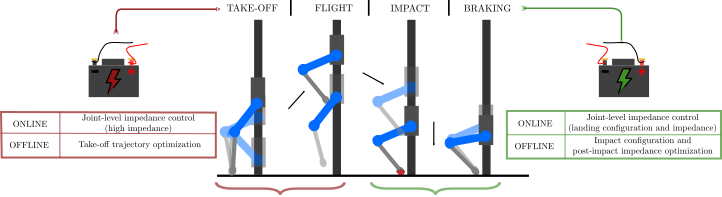
\includegraphics[width=0.9\textwidth]{images/jump_phases_and_pipeline.pdf}
    \caption{A jump sequence decomposed into four main phases, which are synthetically depicted at the center of the figure: the takeoff, the flight, the impact and the braking. During the takeoff phase, energy flows from the power source towards the actuators; after the impact, however, the leg brakes and some of the residual kinetic energy is sent back to the power source and is thus available for regeneration. 
    % Our optimization and control pipeline seeks to exploit these characteristics and, in particular, is made of an offline layer, which houses two separate TO problems, and an online layer, occupied by a simple joint-level impedance controller. 
    }
    \label{fig:pipeline}
\end{figure*}
To be able to perform a jumping task while fully exploiting the capabilities of our prototype, we developed a two-stage pipeline (shown in Fig.~\ref{fig:pipeline}) based on Trajectory Optimization (TO), which in recent years has become one of the most successful methods in generating complex motions for robotic systems\cite{agile_bots::nguyen2019optimized,agile_bots::chignoli2021humanoid, agile_bots::roscia2023orientation}.
% \cite{agile_bots::neunert2017trajectory,agile_bots::winkler2018gait,agile_bots::chignoli2021online,agile_bots::nguyen2019optimized,agile_bots::chignoli2021humanoid, agile_bots::roscia2023orientation,agile_bots::carius2019trajectory}.
Our contributions are the following:
\begin{itemize}
    % \item We explore the jump as a task under several aspects and propose to tackle the problem by grouping together the take-off and flight and impact, braking phase. 
    % \item We enhance our formulations with accurate models for the energy flow from our power source toward the robot.
%    \item The design of a TO problem for jointly addressing the take-off and flight phases, which accounts for several hardware limitations and optimizes for a feasible thrust trajectory, with the objective of maximizing the jump apex height. 
%    Particular care was taken into bridging the gap between optimization and reality. To this purpose, we employ an accurate model of the actuators' dynamics which allows us to introduce meaningful hardware limitations into our formulation.
    % We furthermore elaborate on a series of peculiar characteristics associated with the Inverse Dynamics formulation\cite{to::ferrolho2021inverse} applied to agile Trajectory Generation.
    \item The development of a two-stage TO pipeline for designing and executing jumping maneuvers, while maximizing energy regeneration and impact mitigation, incorporating also accurate actuation and power flow models.
%    The development of a pipeline made of two sequential TOs for the design and execution of jumping maneuvers, incorporating accurate actuation and power flow models, as well as the maximization of energy regeneration and impact mitigation.
%    The first TO handles the thrust phase and generates a feasible take-off trajectory, while accounting for several hardware contraints.  The second TO problem tackles the impact and post-impact breaking phases and employs suitable energy flow and impact dynamics models, which allow us to maximize the energy regenerated by the actuators during braking, while also minimizing the dissipation of kinetic energy due to the impact with the ground.
     In literature, there exists several works reasoning about impact mitigation and energy recuperation, e.g.~\cite{agile_bots::katz2019mini,agile_bots::hawkes2022engineered,agile_bots::chignoli2021humanoid}. However, to the authors' best knowledge, this is the first time the relationship between ground impact and energy regeneration is explored and accounted for \textit{explicitly}  in the context of electrically-actuated robotic jump maneuver design.
    \item The validation of our two TOs and models, both  in simulation and on the real hardware.
\end{itemize}
The rest of the paper is organized as follows. Section~\ref{sec:prb_def} 
%expands upon the peculiarities of jumping maneuvers and
lays down the premises for our approach and TOs. Section~\ref{sec:formulation} details the formulation of our models and optimization problems, focusing on some pivotal aspects specific to the task under analysis, i.e. the jump. Section~\ref{sec:exp_results} shows the results of our study providing experimental validation for the TO formulations. Finally, Section~\ref{sec:conclusions} sums up and comments on the main results of our case study and highlights possible lines of future research.  


\section{Problem framing and state of the art}\label{sec:prb_def}
A jumping task may be split into four main phases (shown in Fig.~\ref{fig:pipeline}): the take-off or thrust, the flight, the impact and the braking. We start by exploring the phases individually and assess the challenges and peculiarities associated with each of them.

During the take-off phase the robot has to accelerate its center of mass (CoM) sufficiently to break the contact from the ground, while modulating the contact forces exchanged with the environment.
% During this phase, the highest amount of energy is drawn from the power source of the robot. 
% Most of the kinetic energy gained during the take-off phase is then converted into potential energy at the apex of the flight phase. 
% When the robot makes contact with the ground, it has already converted a big portion of its potential energy back into kinetic energy at the impact. 
% Based on its distribution among the joints and floating-base, the physical properties of the ground and of the robot's end-effector, part of the kinetic energy may be lost at the impact.
At the impact and while braking, an amount of the available kinetic energy, on the basis of the properties of the colliding bodies (foot and ground) and the configuration of the robot at the impact instant~\cite{impact_dyn::walker1994impact},
may be lost.
% For instance, if considering the specific case of our robot, it is clear that landing with a totally stretched leg on a rigid floor causes all the pre-impact energy to be dissipated through the mechanical structure of the robot, with no residual velocity at the joints after the touchdown.An amount of this kinetic energy, on the basis of the properties of the colliding impact surfaces and on the configuration assumed by the robot at the impact instant~\cite{impact_dyn::walker1990use,impact_dyn::walker1994impact,biomech::cui2021human,impact_dyn::rossi2015pre,impact_dyn::aouaj2021postimpact,impact_dyn::tassi2022impact}, may be lost during the transition from the impact and the braking phase.
% For instance, if considering the specific case of our robot, it is clear that landing with a totally stretched leg on a rigid floor causes all the pre-impact energy to be dissipated through the mechanical structure of the robot, with no residual velocity at the joints after the touchdown.
During the post-impact braking phase, any residual kinetic energy, if available, needs to be somehow dissipated in order to brake the robot. Thus, the question of whether this energy can be harvested or not, instead of being lost in the robot structure and the environment, rises.
% A pivotal aspect which has to be considered when designing and operating legged robot is autonomy: it is crucial for agile maneuvers, when necessary, to be performed with the highest possible efficiency. 
% As we have already highlighted, this principle plays an important role during the take-off, but it also does during the braking phase. 
Looking at nature, it has been highlighted how biological jumpers tend to employ energy storage principles during the landing phases to be able to increase the performance and efficiency of their movements~\cite{biomech::anderson1993storage,biomech::biewener1981elastic}. In the case of our prototype (powered by torque controlled actuators similar to those also used on CENTAURO~\cite{misc::kashiri2019centauro} robot), it is possible to exploit a similar strategy and make use of the power source in place of tendons as temporary energy storage of mechanical energy by performing what is called \textit{energy regeneration}~\cite{reg_braking::yoong2010studies,reg_braking::seok2014design} during braking phases.
% (when this is allowed, like in the case of batteries).
% There are instances of robots designed to mimic the energy storage approach of animals, e.g.~\cite{biomech::hyon2002development}. However, most of the modern robots are powered by electric Brushless Direct Current (BLDC) actuators, like in the case of our prototype.It is well known that it is possible to exploit the Pulse Width Modulation (PWM) power stage of such actuators to perform : by utilizing Field Oriented Control (FOC) it is theoretically possible to send back the negative mechanical energy at the joints during braking back to the power source. 
% In practice, however, there will always be an amount of (resistive) losses between the actuators' phases and the power source, which will inevitably reduce the quota of the recuperated energy. 
% These losses will depend on the amount of quadrature currents produced by the power stage. Intuitively, the faster the breaking is, the higher the torques needed at the link-side and, consequently, the higher the quadrature currents which need to be produced into the motor phases by the power stage. The higher the currents and the higher the ohmic losses inside the motor phases and inside the PWM stage are. 
% While lower braking phase velocities will produce lower regeneration currents and thus result to lower ohmic losses, higher braking phase velocities will produce higher regenerative mechanical energy. 

Based on these considerations, we choose to approach the problem of generating a jumping motion for our prototype in a modular way. Instead of solving a single optimization problem for the whole jump horizon, we split the problem into two separate ones (as shown in Fig.~\ref{fig:pipeline}) to gain simplicity both in terms of formulation and computational complexity. We tackle the take-off and flight phases (up to the apex) in the first one, with the objective of maximizing the apex height, while we address the remaining phases in the second. Given the characteristics of the torque controlled actuation used to power our robot leg we employ a joint space impedance controller to track the references provided by our take-off TO. For the landing phase, we restrict our attention to a specific breaking strategy: after the apex, the joint level impedance controller is fed with desired landing impedance set points and a fixed reference configuration. The main idea for the braking phase is to see if it's possible to optimize the impedance gains and configuration to maximize the recovered energy while also preventing high impacts.
% However, the two groups of phases $\{\text{take-off, flight}\}$ and $\{\text{impact, braking}\}$ cannot be independent and we hence need a way to couple them. We achieve this is a very straightforward way by employing the solution of the first and, in particular, the achieved tip jump height, to estimate the pre-impact velocity. The pre-impact velocity is then used as an input parameter for the braking TO.

%During the post-impact braking phase, any residual kinetic energy, if available, needs to be somehow dissipated in order to brake the robot. The question of whether this energy can be harnessed or not, instead of being lost in the robot structure and the environment, rises.
% A pivotal aspect which has to be considered when designing and operating legged robot is autonomy: it is crucial for agile maneuvers, when necessary, to be performed with the highest possible efficiency. 
% As we have already highlighted, this principle plays an important role during the take-off, but it also does during the braking phase. 
%Looking at nature, it has been highlighted how biological jumpers tend to employ energy storage principles during the landing phases to be able to increase the performance and efficiency of their movements~\cite{biomech::anderson1993storage,biomech::biewener1981elastic,biomech::biewener1998muscle,biomech::konow2012muscle}. In the case of our prototype (powered by the series elastic actuators also used on the CENTAURO~\cite{misc::kashiri2019centauro} robot), it is possible to exploit a similar strategy and make use of the power source in place of tendons as temporary energy storage of mechanical energy by performing what is called \textit{energy regeneration}~\cite{reg_braking::yoong2010studies,reg_braking::kivanc2016regenerative,reg_braking::riyadi2019analysis,reg_braking::seok2014design}.
% (when this is allowed, like in the case of batteries).
% There are instances of robots designed to mimic the energy storage approach of animals, e.g.~\cite{biomech::hyon2002development}. However, most of the modern robots are powered by electric Brushless Direct Current (BLDC) actuators, like in the case of our prototype.It is well known that it is possible to exploit the Pulse Width Modulation (PWM) power stage of such actuators to perform : by utilizing Field Oriented Control (FOC) it is theoretically possible to send back the negative mechanical energy at the joints during braking back to the power source. 
%In practice, however, there will always be an amount of (resistive) losses between the actuators' phases and the power source, which will inevitably reduce the quota of recoverable energy. 
% These losses will depend on the amount of quadrature currents produced by the power stage. Intuitively, the faster the breaking is, the higher the torques needed at the link-side and, consequently, the higher the quadrature currents which need to be produced into the motor phases by the power stage. The higher the currents and the higher the ohmic losses inside the motor phases and inside the PWM stage are.
%Consequently, the braking phase needs to be sufficiently slow to avoid large ohmic losses and hardware limits, but also fast enough to produce sufficient regenerative mechanical energy. 

% \section{Contributions}\label{sec:contrib}

On the basis of the qualitative analysis of the problems and of the main aspects related to jumping with robots which is outlined in Sec.~\ref{sec:prb_def}
The pipeline is made of an online and an offline layers (see Fig.~\ref{fig:pipeline}). The online layer is occupied by a simple yet-effective joint level impedance controller, while the offline layer is made of two separate TO problems. The first one addresses the take-off and flight phases, while the second one tackles the impact and braking phases. Our choice of grouping together the first and last two phases of a jump stems very naturally from the considerations highlighted in Sec.~\ref{sec:prb_def}. Furthermore, we choose to exploiting Trajectory Optimization (TO), which has become one of the most successful methods for generating complex motions of robotic systems\cite{agile_bots::neunert2017trajectory,agile_bots::winkler2018gait,agile_bots::chignoli2021online,agile_bots::nguyen2019optimized,agile_bots::chignoli2021humanoid, agile_bots::roscia2023orientation,agile_bots::carius2019trajectory} in recent years, due to its potential in accounting for the performance of the hardware. The benefits of TO are well-known: stability, robustness and interpretability.

\section{Formulation}\label{sec:formulation}
\subsection{System modeling}
The dynamics of a general floating-base system can be written as
\begin{equation}\label{eq:rigid_body_dyn}
B(q)\,\dot{v} +C(q, v)\,v + g(q) = \tau_{a} + J^T\,f
\end{equation}
where $B\in\mathbb{R}^{n_v\times n_v}$ and $C\in\mathbb{R}^{n_v\times n_v}$ are, respectively, the generalized inertia and Coriolis matrices of the system; $q\in\mathbb{R}^{n_q}$ and $v\in\mathbb{R}^{n_v}$ are the configuration and generalized velocity vectors of the system, while $g\in\mathbb{R}^{n_v}$ and $\tau_a=\begin{bmatrix}
0_{6\times 1};
\tau_{\mathrm{m}}
\end{bmatrix}\in\mathbb{R}^{n_v}$ are, respectively, the generalized gravity vector and the actuation torques. Finally, $J^T(q)\,f$ are the torques generated by the generalize wrench $f$ through the contact jacobian $J$. In the specific case of our leg prototype, the system has a degenerate floating base with only a single degree of freedom, given by the sliding guide joint (see Fig.~\ref{fig:jumping_sequence}); as a consequence, $\tau_a$ is simply $\begin{bmatrix}
0;\,\tau_{\mathrm{m}}\end{bmatrix}$, $n_q = n_v = 3$, $J\in\mathbb{R}^{3\times 3}$ and $f\in\mathbb{R}^3$, if we only consider a point contact with the ground.

\subsection{Actuator modeling: quadrature current estimation}
% As already highlighted in Sections~\ref{sec:introduction} and ~\ref{sec:prb_def}, jumping motions are particularly demanding for the robot. In particular, the high torques required to perform the take-off and to stop the robot after the impact have to be produced by the Brushless Direct Current (BLDC) actuators of the leg. 
It is known~\cite{foc::krause2013analysis} that the torque-quadrature current characteristic for Brushless Direct Current (BLDC) actuators is well approximated by the relationship
\begin{equation}\label{eq:torque_iq}
\tau_m = K_t\,i_q
\end{equation}
with the $K_t\in\mathbb{R}$ is the torque constant of the motors.
% Hence, high driving torques need to be produced by high quadrature currents. This two quantities cannot assume, however, arbitrarily large values, due to both mechanical and electrical limitations. Even if our prototype is equipped with current (and torque) sensors, in order to preemptively avoid damage to the hardware, it is also crucial to embed an estimate model of the actuators into our TO formulations.
% We start by writing the motor-side dynamics for a single actuator as in~\cite{friction_comp::le2008friction}:
% \begin{equation}\label{eq:rotor_dyn}
%     \tau_m + \tau_r = I_r\,\dot{v}_m
% \end{equation}
% where $\tau_m$ is the driving torque acting on the rotor, $\tau_r$ includes all torques coming from the reduction stage of the actuator. $I_r$ is the rotational inertia of the rotor and $\dot{v}_m$ is acceleration of the rotor. If no losses are present between the robot and the link side, $\tau_r$ is simply equal to the torques measured at the link, reflected to the motor (through the reduction ratio). However, when working with non direct-drive actuators, there will always be an amount of losses in the reduction stage. This was especially true in our case, where the actuators posses a reduction ratio of $1:50$ and there is a relevant amount of friction at the joints.
Employing this information, we can write a friction-compensated version of the rotor-side dynamics as in~\cite{friction_comp::le2008friction}:
\begin{equation}\label{eq:rotor_dyn_friction}
    K_t\,i_q  - \tau_l\,\eta + 
\tau_{\mathrm{fl}} \, \eta = I_r\,\dfrac{\dot{v}_l}{\eta}
\end{equation}
where $\tau_l\in\mathbb{R}^{2}$ are the link side torques acting on the actuators, $\tau_{\mathrm{fl}}\in\mathbb{R}^{2}$ is a vector modeling the friction torques reflected at the link-side, $i_q\in\mathbb{R}^{2}$ are the quadrature currents, $0 < \eta \leq 1$ is the reduction ratio from the motor to link side and $I_r$ is the axial inertial of the rotor. Equation~\eqref{eq:rotor_dyn_friction} can be used to build a friction observer (as done in~\cite{friction_comp::le2008friction}) or, alternatively, can be employed to calibrate a suitable friction model for $\tau_{\mathrm{fl}}$.
% The availability of such a model, as already highlighted, will be crucial in enforcing realistic constraints into our TO formulation. 
Specifically, we use the simple Coulomb-like friction model 
\begin{equation} \label{eq:friction_torque}
\tau_{\mathrm{fl}} = - K_{\mathrm{f, s}}\,\mathrm{signh}({v_l}) - K_{\mathrm{f, d}}\,v_l
\end{equation}
where $\mathrm{signh}()$ is a smooth approximation of the sign function based on the hyperbolic tangent and the scalars $K_{\mathrm{f, s}}$ and $K_{\mathrm{f, d}}$ are the static and dynamic friction coefficients respectively. We employ~\eqref{eq:rotor_dyn_friction} to estimate the friction coefficients in~\eqref{eq:friction_torque} by solving a simple least-squares regression problem with data collected during suitable calibration trajectories. Figure~\ref{fig:iq_model_tracking} shows the tracking performance of the resulting calibrated model w.r.t. actual measurements.
\begin{figure}
    \centering
    \includegraphics[width=1.0\columnwidth]{images/iq_tracking.pdf}
    \caption{Validation of the quadrature current $i_q$ model during a simple test: the leg stands on the ground with low-joint impedance and a vertical pushing force is applied to the base link. The tracking of the calibrated model is accurate, thus justifying its incorporation into our TO formulation.}
    \label{fig:iq_model_tracking}
\end{figure}
\subsection{Take-off optimization: maximizing the reached apex height}\label{subsec:takeoff_opt}
% \begin{figure}
%     \label{fig:ref_vs_res}
%     \centering
%     \includegraphics[width=1\columnwidth]{images/defects_full_with_zoom.pdf}
%     \caption{Importance of the refinement step for the take-off TO formulation. The re-sampled solution, shown as dotted lines, has relevant dynamic defects on the floating base (i.e. the sliding guide). The force on that joint should be $0$ for a feasible solution. On the contrary the solution of the refined problem has $0$ defects. Also, note how the CoM trajectory of the refined solution is different.}
% \end{figure}
Given the scope of our case study, we are interested in performing the jumping task with the highest performance our prototype is able to offer. For a jumping trajectory, this means maximizing the height at the apex of the jump, while accounting for the hardware's constraints. To achieve this, we employ an inverse dynamics-based formulation and hence use accelerations $\dot{v}$ and contact forces $f$ as inputs to the rigid body dynamics~\eqref{eq:rigid_body_dyn}. The benefits of employing inverse-dynamics based formulations, as opposed to forward-dynamics based ones, are starting to become apparent~\cite{to::ferrolho2021inverse},~\cite{to::mastalli2022inverse}: an increased numerical efficiency and stability, particularly for coarse discretizations. We define the states and inputs vectors $x_t$ and $u_t$ of  our take-off TO as
\begin{eqnarray}
&x_t = \left[q,~v,~\dot{v},~f\right]\label{eq:states_takeoff_opt}\\
&u_t = \left[\ddot{v},~\dot{f}\right]\label{eq:inputs_takeoff_opt}
\end{eqnarray}
The running cost of the TO is formulated as
\begin{dmath}\label{eq:takeoff_running_cost}
    \ell_{t}(x_t,~u_t) = \ell_f + \ell_{\dot{f}} + \ell_{v} +  \ell_{\dot{v}} + \ell_{\ddot{v}}
\end{dmath}
where the weighted costs $\ell_{f}$, $\ell_{\dot{f}}$, $\ell_{v}$, $\ell_{\dot{v}}$, $\ell_{\ddot{v}}$ are all quadratic in, respectively, $f$, the yank $\dot{f}$, $v$, $\dot{v}$ and the jerk $\ddot{v}$. 
The cost for the maximization of the CoM height $h_{\mathrm{CoM}}$ is implemented as a terminal constraint at the apex time $T_{\mathrm{apex}}$ of the form 
\begin{equation}\label{eq:max_com}
\ell_{\mathrm{CoM}}^F(T_{\mathrm{apex}}) = \dfrac{1}{h_{CoM}(q(T_{\mathrm{apex}})) + \epsilon}
\end{equation}
where $\epsilon$ is a small positive number to avoid singularities.
The only non-linear cost is the term $\ell_{\mathrm{CoM}}$, which maximizes the height of the CoM. The integral cost of the take-off TO can hence be written as
\begin{dmath}\label{eq:takeoff_opt_L}
    L_{t} \left( W_t\right) = \ell_{\mathrm{CoM}}^F + \int_{0}^{T_{\mathrm{apex}}}\,\ell_{t}(\tau)\,d\tau
\end{dmath}
where
\begin{equation}\label{takeoff_opt:opt_vars}
W_t \coloneqq \left[x_t,~u_t,~T_{\mathrm{takeoff}},~T_{\mathrm{apex}}\right]
\end{equation} 
collects our optimization variables and $T_{\mathrm{takeoff}}$ and $T_{\mathrm{apex}}$ represent, respectively, the take-off and apex instant. 
The cost function~\eqref{eq:takeoff_opt_L} is complemented by a set constrains, which are used to  enforce both the jumping maneuver and a series of crucial hardware constraints. First, defining $\tau_{\mathrm{lim}}$ as the actuated joints torque limits, we impose bounds on the torques $\tau_a$:
\begin{equation}\label{eq:tau_lims}
- \begin{bmatrix}
0\\
\tau_{\mathrm{lim}}
\end{bmatrix} \leq \tau_a \leq \begin{bmatrix}
0\\
\tau_{\mathrm{lim}}
\end{bmatrix}
\end{equation}
Furthermore we constrain the tip to stay on the ground before the takeoff instant with the following couple of constraints, respectively, on the tip position $\chi_{\mathrm{tip}}$ and velocity $\dot{\chi}_{\mathrm{tip}}$
\begin{eqnarray}
&\chi_{\mathrm{tip, z}} = 0 \label{eq:tip_on_ground}\label{eq:tip_on_ground_vel};~t = 0\\
&\dot{\chi}_{\mathrm{tip}} = 0;~t\in\left[0, T_{\mathrm{takeoff}}\right]
\end{eqnarray}
We also impose the apex at the final instant with the terminal constraint
\begin{equation}\label{eq:apex_com}
\dot{\chi}_{\mathrm{CoM, z}} = 0;~t = T_{\mathrm{apex}}
\end{equation}
% The flight phase is imposed by constraining the contact force to be null after the takeoff, up to the final instant. Furthermore $f$ should always be positive and its tangential component $f$ should lie inside the friction pyramid defined by the coefficient~$\mu$ and the tangential an normal components $f_t$ and $f_n$. Summing up:
We impose contact and friction contraints on $f$ with
\begin{eqnarray}\label{eq:f_cnstrnt}
&f \geq 0;~t\in\left[0, T_{\mathrm{takeoff}}\right] \label{eq:f_positive} \\
&f = 0; ~t\in\left[T_{\mathrm{takeoff}}, T_{\mathrm{apex}}\right] \\
&-\mu\,f_n \leq f_t\leq \mu\,f_n;~t\in\left[0, T_{\mathrm{takeoff}}\right] 
\end{eqnarray}
At the first instant, the leg should also start still; as a consequence
\begin{equation}\label{eq:starts_still}
    v = 0;~t = 0
\end{equation}
We also account for the calibrated actuation model~\eqref{eq:rotor_dyn_friction} by constraining the quadrature current $i_q$ of the actuator as
\begin{eqnarray}
&K_t\,i_q  - \tau_{l}\,\eta + 
\tau_{\mathrm{fl}} \, \eta = I_r\,\dfrac{\dot{v}_l}{\eta}\label{eq:rotor_dyn_friction_cnstrnt}\\
&- i_{q, \mathrm{max}} \leq i_q \leq i_{q, \mathrm{max}}\label{eq:rotor_dyn_friction_cnstrnt2}
\end{eqnarray}
Finally, we can write the continuous version of our take-off TO as
\begin{subequations}\label{eq::takeoff_opt_prb}
	\begin{dmath}
		\min_{W_t}~L_{t}\left(W_t \right)
	\end{dmath}
	\centering\text{subject to}
	\begin{eqnarray}
	&\text{rigid body dynamics}~\eqref{eq:rigid_body_dyn}
    \label{eq:rigid_body_dyn_cnstrnt}\\
    &~\text{constraints}~\text{~\eqref{eq:tau_lims}~to~ \eqref{eq:rotor_dyn_friction_cnstrnt2}} \\
    &\text{joint position and velocity ranges}
	\end{eqnarray}
\end{subequations} 

The continuous TO problem described by~\ref{eq::takeoff_opt_prb} is then transcribed over a grid of $N$ nodes by employing the multiple shooting method~\cite{to::bock1984multiple}. The solution to the discretized version of~\eqref{eq::takeoff_opt_prb} is first re-sampled at a desired constant rate following the procedure detailed in~\cite{to::horizon_to} and then fed as initial guess to a \textit{refined} discretized problem with the same costs and constraints as~\eqref{eq::takeoff_opt_prb}, but with fixed time intervals. This procedure, very similar to the \enquote{mesh refinement} employed in~\cite{to::horizon_to}, is needed to make the re-sampled solution dynamically feasible. As shown in~\cite{to::horizon_to}, in fact, the re-sampling procedure may introduce large dynamics defects on the floating-base of the robot, thus making the obtained solution dynamically unfeasible. 
As an additional remark, the authors would like to underline the importance of the terms $\ell_{\dot{f}}$ and $\ell_{\ddot{v}}$ in minimizing the feasibility gap between simulation and reality.
\begin{figure}[t]
    \centering
    \includegraphics[width=1\columnwidth]{images/inv_dyn_caveat.pdf}
    \caption{Joint accelerations (on top) and normal component of the ground reaction force obtained for a refined take-off problem without jerk and yank minimization: the solver exploits a caveat in the inverse dynamics formulation and finds a solution which respects node constraints, but is not feasible in reality.}
    \label{fig:inv_dyn_caveat}
\end{figure}
Fig.~\ref{fig:inv_dyn_caveat} shows the results of a refined solution where the regularization costs on the jerk $\ddot{v}$ and the yank $\dot{f}$ are not employed. Looking at the picture, the solver exploits a caveat in the inverse dynamics-based formulation and produces an impulse of $f$ at the takeoff-instant without violating the inverse dynamics on the nodes. It does so by compensating with corresponding impulses of $\dot{v}$. This acceleration and ground reaction forces are however not feasible in reality, and this could be checked by looking at the dynamics residuals obtained by re-sampling the refined trajectory at a higher rate. This shows how with the inverse dynamics-based formulation applied to highly dynamic TO needs to be complemented with suitable regularization of the jerk $\dot{v}$ and $\dot{f}$ to function properly.
\subsection{Landing phase: impact dynamics modeling}\label{subsec:impact_min}
\begin{figure}[t]
    \centering
    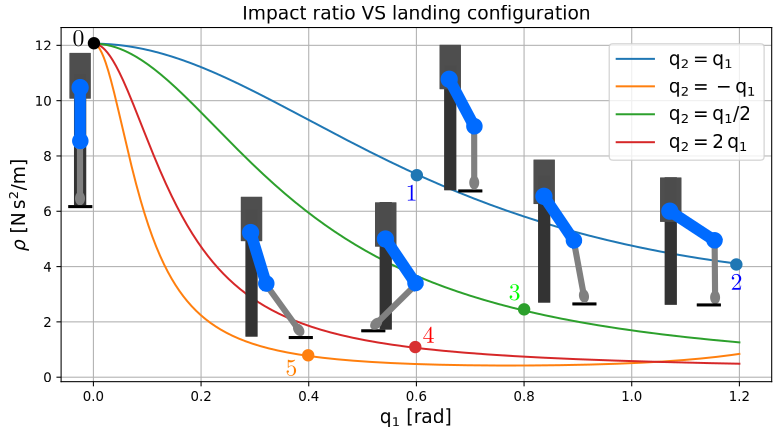
\includegraphics[width=1\columnwidth]{images/impact_ratio.pdf}
    \caption{Depending on the landing configuration, the impact felt by the robot at the ground can vary greatly. In this figure, we show how the impact ratio $\rho$ changes with the landing configuration, which is described by the two joint variables $q_1$ and $q_2$. We specifically highlight 6 representative configurations, which are shown on top of the impact curves.}
    \label{fig:impact_ratio}
\end{figure}
After the apex of the flight phase, the leg will make contact with the ground. Under the usual assumption that the impact duration is negligible with respect to the time scale over which the body dynamics evolves, it is possible to integrate~\eqref{eq:rigid_body_dyn} over the impact instant to obtain the so called \textit{impact dynamics}~\cite{impact_dyn::walker1990use}:
\begin{equation}
    \label{eq:impact_dyn}
B(\hat{q})\,\left[v_{+} - v_{-}\right] = J^{T}(\hat{q})\,\hat{f}
\end{equation}
where $\hat{q}$ is the impact configuration of the robot, $v^{+}$ and $v^{-}$ are the post-impact and pre-impact generalized velocities of the system and $\hat{f}$ is the impact impulse, defined as the integral of the impact force during the impact interval.
The forward kinematics continues to be valid at the impact instant, so we can write
\begin{equation}\label{eq:imp_forw_dyn}
    J\,\left( v^{+} - v^{-} \right) = \dot{\chi}_{\mathrm{tip}}^{+} - \dot{\chi}_{\mathrm{tip}}^{-}
\end{equation}
where the explicit dependence upon $\hat{q}$ is dropped for simplicity and $\dot{\chi}_{\mathrm{tip}}$ is the cartesian velocity of the end-effector. 
Looking at equations~\eqref{eq:impact_dyn},~\eqref{eq:imp_forw_dyn} we see that the result of the impulse $\hat{f}$ is to produce a step in the joint velocities $v$ which, in turn, will produce a step in the end-effector velocity. 

Let us look at the energetic aspect of the impact, which is particularly relevant for our case study. The variation of kinetic energy right before and after the impact is given by the simple analytical relationship
\begin{dmath}\label{eq:delta_e_k}
    \Delta E_k = E_k^{+} - E_k^{-} = \dfrac{1}{2}\,\left({v^{+}}^T\,B\,v^{+} - {v^{-}}^T\,B\,v^{-}\right)
\end{dmath}
From~\eqref{eq:impact_dyn}, exploiting the non-singularity of $B$, we can write
\begin{equation}\label{eq:v_plus}
v^+ = B^{-1}\,J^T\,\hat{f} + v^{-}
\end{equation}
where we recall that $B$ is the generalized inertia matrix of the system~\eqref{eq:rigid_body_dyn}.
Substituting~\eqref{eq:v_plus} into~\eqref{eq:delta_e_k} and~\eqref{eq:imp_forw_dyn}, after a little rearranging, we can obtain the alternative expression
\begin{dmath}\label{eq:delta_e_k_altern}
    \Delta E_k = \dfrac{1}{2}\,\hat{f}^T\,\left(\dot{\chi}_{\mathrm{tip}}^{+} + \dot{\chi}_{\mathrm{tip}}^{-}\right)
\end{dmath}
From~\eqref{eq:delta_e_k} it is clear that, in general, energy is not conserved at the impact. As a simplification, we assume an inelastic impact with the ground (which is a good approximation for the setup shown in Fig.~\ref{fig:jumping_sequence}) and the velocity of the actuated joints to be negligible w.r.t. the linear guide velocity. This second assumption was successfully verified both in simulation and on the hardware over several jumping tests. With these premises, we can write a simplified version of~\eqref{eq:imp_forw_dyn} and~\eqref{eq:delta_e_k} for our specific case as
\begin{dmath}\label{eq:imp_forw_dyn_simpl}
    J\, v^{+} - J\, v^{-}_{*} = - \dot{\chi}_{\mathrm{tip}}^{-}
\end{dmath}
and 
\begin{dmath}\label{eq:delta_e_k_simpl}
    \Delta E_k = \dfrac{1}{2}\,\hat{f}^T\, \dot{\chi}_{\mathrm{tip}}^{-}
\end{dmath}
with 
\begin{equation} \label{eq:chi_dot_simpl}
    \dot{\chi}_{\mathrm{tip}}^{-} = \left[0, 0, 
v_{\mathrm{fall}}\right]
\end{equation}
and 
\begin{equation} \label{eq:v_m_star}
    v^{-}_{*} = \left[v_{\mathrm{fall}, 0, 0}\right]
\end{equation}
where $v_{\mathrm{fall}}$ is the vertical component of the velocity vector right before the impact.
Furthermore, we can also speculate, being the fall vertical, that most of the impulse will be concentrated on the vertical component of $\hat{f}$. As a consequence, 
\begin{equation}\label{eq:f_hat_simpl}
    \hat{f} = \begin{bmatrix}
0\\
0\\
\hat{f}_{n}
\end{bmatrix}
\end{equation}
and we can therefore conclude that, since $v_{\mathrm{fall}} \leq 0$ and $f_n > 0$ for a vertical fall, $\Delta E_{k} \leq 0$. 
Under our assumptions of inelastic and vertical impact, it is possible to combine the impact equations and arrive, after a bit of manipulation, to the following relationship between the normal component of the impact impulse and the pre-impact velocity~\cite{impact_dyn::tassi2022impact}:
\begin{equation}\label{eq:impact_ratio}
    \rho \coloneqq \dfrac{\hat{f}_n}{v_{\mathrm{fall}}} = -\dfrac{1}{\Lambda^{-1}_{2,2}(\hat{q}_1, \hat{q}_2)}
\end{equation}
to which, from now on, we will refer to as the \enquote{impact ratio}. $\Lambda^{-1}_{2,2}$ is the third element on the diagonal of the inverse cartesian inertia matrix $\Lambda^{-1} = J\,B^{-1}\,J^{T}\in\mathbb{R}^{3\times3}$. For our simple case in which the floating joint can only move vertically, $\rho$ only depends on the configuration of the leg at the impact $\left[\hat{q}_1,\hat{q}_2 \right]$.
Since we cannot know exactly when the impact will happen, $v_{\mathrm{fall}}$ cannot be used to reduce the dissipation of kinetic energy. The only option is to reduce $\hat{f}$ or, equivalently, $\rho$, which we know will depend on the landing configuration. 
Exploiting the simplicity of~\eqref{eq:impact_ratio}, we can have a quantitative glimpse at how the impact varies depending on the landing configuration. This is exactly what is shown in Fig.~\ref{fig:impact_ratio}. Most notably, the configuration n.$0$ is the absolute worst in terms of impact: all the kinetic energy is dissipated at the impact through the ground and, more importantly, through the robot itself. As a consequence, without choosing properly the landing configuration, we could potentially endanger the mechanical integrity of the robot and drastically reduce the energy available for regeneration during the braking phase.
\subsection{Landing phase: energy regeneration}\label{subsec:energy_reg}
\begin{figure}[t]
    \centering
    \includegraphics[width=1\columnwidth]{images/dropdown_const_imp.pdf}
    \caption{Results of the dropdown tests performed in simulation, with fixed joint impedance. The leg is dropped from an height (of the tip w.r.t. to the ground) of $0.5\mathrm{m}$ multiple times with 6 different touchdown configurations chosen manually on the curve~\ref{fig:impact_ratio} (the same shown in Fig.~\ref{fig:impact_ratio}). At each touchdown, the regenerative energy flow $e_{\mathrm{reg}}$ towards the power source is monitored using the model~\eqref{eq:energy_flow}. The results indicate that not all configurations with low impact are equivalently suitable for energy recuperation.}
    \label{fig:fixed_imp_reg_energy}
\end{figure}
\begin{figure}[t]
    \centering
    \includegraphics[width=1\columnwidth]{images/dropdown_const_landing.pdf}
    \caption{Results of the dropdown tests performed in simulation, with the landing configuration fixed to the n.~$4$ (shown in Fig.~\ref{fig:impact_ratio}). The leg is dropped from an height (of the tip w.r.t. to the ground) of $0.5\mathrm{m}$ multiple times with 4 different joint impedance setpoints. At each touchdown, the regenerative energy flow $e_{\mathrm{reg}}$ towards the power source is monitored using the energy model~\eqref{eq:energy_flow}. The results confirm that landing with stiff joints greatly diminishes the amount of energy recovered. On the contrary landing with \enquote{soft} joints diminishes the joule losses inside the actuators, due to the lower required braking torques.}
    \label{fig:fixed_conf_reg_energy}
\end{figure}

In Section~\ref{sec:prb_def} we have already qualitatively highlighted how during the braking phase it is possible to recover some of the post-impact residual energy. Here we briefly outline the formulation of a simple and effective model of the energy flow from the power source (in our case a battery) and the actuators, which will be employed in the braking TO problem outlined in the upcoming Section~\ref{subsec:energy_rec_opt}. 

When performing Field Oriented Control on BLDC motors (like in our case), it is possible to write the power balance from the battery towards the actuators in the so called \textit{qd0} reference frame employing the Park transform~\cite{foc::krause2013analysis} as 
\begin{equation}\label{eq:power_balance}
    p_{\mathrm{batt}} = - \dfrac{3}{2}\,\left(R\,i_{q}^2 + L_q\,i_{q}\,\dfrac{d}{dt}\,i_q\,\right) - K_t\,i_q\,v_m
\end{equation}
where $R$ and $L_q$ are the phase resistance and quadrature inductance of the motors and $v_m$ is the rotor velocity. The relationship, for simplicity, is shown for a single actuator. Equation~\eqref{eq:power_balance} can be integrated over an arbitrary interval of time to obtain the energy flow as 
\begin{dmath} \label{eq:energy_flow}
e_{\mathrm{batt}}(t) = e_{\mathrm{batt}}(t_0)- \dfrac{3}{2}\,R\,\int_{t_0}^{t}\,i_{q}^2\,d\tau\,- \dfrac{3}{4}\,L_q\,\left[i_q^2(t) - i_q^2(t_0)\right]\,-\,K_t\,\int_{t_0}^{t}\,i_q\,v_{m}\,d\tau
\end{dmath}
Inside~\eqref{eq:energy_flow} we can distinguish, in this order, the initial energy level of the battery, the dissipative joule losses, a conservative term representing the energy stored inside the motor phases and the mechanical energy at the motor rotor. For our purposes, the inductive term in~\eqref{eq:energy_flow}, which is conservative and also weighted by $L_q$ (usually in the order of $\mu\,\mathrm{H}$), can be neglected. 

Figures~\ref{fig:fixed_imp_reg_energy} and~\ref{fig:fixed_conf_reg_energy} report data from two series of dropdown tests performed in simulation while monitoring the energy flow with~\eqref{eq:energy_flow}. The leg, while being controlled by a joint-space impedance control, is dropped from an height on $0.5\mathrm{m}$ multiple times with different configurations and different joint impedance setpoints. After each touchdown, the energy recovered is evaluated using~\eqref{eq:energy_flow}. The results show that not all low-impact configurations are suitable for energy regeneration and that the amount of recovered energy is indeed also influenced greatly by the employed joint impedance setpoints. 
\begin{figure}
    \centering
    \includegraphics[width=1.0\columnwidth]{images/reg_pow_tracking.pdf}
    \caption{Validation of the model of the power flow model: the leg stands on the ground with low-joint impedance and an vertical oscillating force is applied to the base link. Looking at the plot, we can confirm that the model is indeed accurate in predicting the power flow of our setup.}
    \label{fig:reg_pow_model_tracking}
\end{figure}
The model~\eqref{eq:power_balance} was also successfully validated on the real hardware by employing a suitable power sensing setup. The results of the validation are shown and briefly discusses in Fig.~\ref{fig:reg_pow_model_tracking}. 
\subsection{Post-impact optimization: minimizing impact impulse and maximizing energy recovery}\label{subsec:energy_rec_opt}
Motivated by the results shown in Fig~\ref{fig:fixed_conf_reg_energy} and~\ref{fig:fixed_imp_reg_energy} and~\ref{fig:impact_ratio}, we formulate a suitable TO to jointly address the impact and power regeneration during the braking phases. As done in Sec~\ref{subsec:takeoff_opt} we employ an inverse dynamics-based formulation. In this case, the running cost takes the form
\begin{dmath}\label{eq:takeoff_running_cost_braking}
    \ell_{b}(x_b, u_b) = \ell_{p_{\mathrm{batt}}} + \ell_f + \ell_{\dot{v}}
\end{dmath}
where
\begin{eqnarray}
    x_b = \left[q,\,v\right]\\
    u_b = \left[\dot{v},\,f\right]
\end{eqnarray}
and $\ell_f$ and $\ell_{\dot{v}}$ are simple weighted quadratic regularizations on the inputs. In this case, being the braking a less dynamic phase than the take-off, we don't employ the additional regularization terms on the $\ddot{v}$ and $\dot{f}$ (see Sec.~\ref{subsec:takeoff_opt}). The weighted stage cost $\ell_{p_{\mathrm{batt}}}$ is build using directly $- p_{\mathrm{batt}}$~\eqref{eq:power_balance} and neglecting the inductive term. 
Differently from before, we formulate the problem with a fixed phase duration $T_f$ and impose the impact dynamics laws of Section~\ref{subsec:impact_min} only at the initial instant of the optimization horizon, where $v^{-}$~\eqref{eq:impact_dyn} assumes the role of a parameter of the problem. To encourage impact mitigation, we use a weighted initial cost $\ell_{\Delta E_k}^{I}$, based directly on~\eqref{eq:delta_e_k}. We furthermore use a simple weighted quadratic terminal cost $\ell_{v}^F$ to promote low velocities at the end of the horizon (the leg needs to break).
% \begin{eqnarray}\label{eq:reg_v}
%     % &\ell_{v, i} = \dfrac{1}{v(0)^T\,v(0) + \epsilon}\\
%     &\ell_{v, f} = v^T(T_f)\,v(T_{f})
% \end{eqnarray}
% The first term helps the solver not to get stuck in the local minima of the straight leg landing configuration n.$[0]$: looking at Figure~\ref{fig:impact_ratio}, the slope of the impact curve near the origin is small, which could cause slow convergence issues. The second term $\ell_{\dot{v}, f}$ is a simple quadratic cost to promote low velocities at the end of the horizon (the leg needs to break).
Once again, we employ the ground contact and force constraints ~\eqref{eq:tip_on_ground},~\eqref{eq:f_positive}, this time on the whole TO horizon. More importantly, we impose a joint impedance controller with
\begin{eqnarray}\label{eq:imp_cntrl}
    \tau_{l} - K_p\,\circ\,\left(q_{l} - \hat{q}\right) - K_d\,\circ\,\left(\dot{q}_{l} - 0 \right)= 0 
\end{eqnarray}
where $\tau_{l}$, $q_{l}$, $\dot{q}_{l}$ refer to the actuated joint only, $K_p\in\mathbb{R}^{2}$ and $K_d\in\mathbb{R}^{2}$ are, respectively, stiffness and impedance gain vectors, which are to be optimized and $\hat{q}$ is the reference configuration for the impedance controller, which is kept constant through the horizon and equal to the landing configuration. The symbol $\circ$ is used to indicate the element-wise product between the operands.
Our final braking problem takes the form
\begin{subequations}\label{eq::braking_opt_prb}
	\begin{dmath}
		\min_{W_{b}}~L_{b}\left(W_{b}\right)
	\end{dmath}
	\centering\text{subject to}
	\begin{eqnarray}
	&\text{rigid body dynamics}~\eqref{eq:rigid_body_dyn}\\
    &\text{foot tip contact}~\eqref{eq:tip_on_ground},~\eqref{eq:f_positive}~\text{up to}~T_f\\
    &\text{joint impedance control}~ \eqref{eq:imp_cntrl} \\
    &\text{torque limits}~\eqref{eq:tau_lims}\\
    &\text{impact dynamics}~\eqref{eq:impact_dyn};~t = 0\\
    &\text{post-impact velocity:}~v^{+} = v;~t = 0\\
    &\text{landing configuration: }~q = \hat{q};~t=0\\
    &\text{joint position and velocity ranges}	\end{eqnarray}
\end{subequations} 
where
\begin{dmath}
    W_{b} = \left[x_b,\,u_b,\,K_p,\,K_d,\,\hat{q}\right]
\end{dmath}
are our optimization variables and
\begin{dmath}\label{eq:takeoff_opt_L_b}
    L_{b} \left( W_b\right) = \ell_{\Delta E_k}^{I} + \int_{0}^{T_f}\,\ell_{b}(\tau)\,d\tau + \ell_{v}^F
\end{dmath}
is the employed cost function.
% It should be noted that we could have inverted~\eqref{eq:impact_dyn} and obtained analytical expressions for the relationships between $v^{+} - v^{-}$ and $i$ or $\chi_{\mathrm{tip}}^{+} - \chi_{\mathrm{tip}}^{-}$ and $i$ as done in~\cite{impact_dyn::walker1994impact}, but this would require the introduction of the well-known \textit{cartesian inertia matrix} $\Lambda\,\coloneqq \left(J\,B^{-1}\,J^{T}\right)$. This in turn, would need the computation of $B^{-1}$, which would reintroduce the issues related to forward dynamics formulations~\cite{to::ferrolho2021inverse}. 
The only parameter over which~\eqref{eq::braking_opt_prb} depends is the pre-impact velocity $v^{-}$ (through the impact dynamics constraint~\eqref{eq:impact_dyn}) which, under the simplifications outlined in Sec.~\ref{subsec:impact_min}, can be approximated with~\eqref{eq:v_m_star}. Given the apex tip height $h_{\mathrm{tip}}$ provided by the solution of~problem~\eqref{eq::takeoff_opt_prb}, we can compute a reasonable estimate for $v^{-}$ as $[-\sqrt{2\,g\,h_{\mathrm{tip}}},~0,~0]$, where $g$ is the acceleration of gravity.


% \section{Simulation results}\label{sec:sim_results}

\section{Results}\label{sec:exp_results}
The TO optimization problems~\eqref{eq::takeoff_opt_prb} and~\eqref{eq::braking_opt_prb} are conveniently written employing the API provided by the Horizon tool~\cite{to::horizon_to} and solved on a 11th Gen Intel(R) Core(TM) i7-11800K CPU, using Ipopt and MA57 linear solver for  step computations. 
The obtained optimal results are then tested both in simulation and on the real hardware.
%showcasing the efficacy of our formulation in capturing the characteristics of the hardware. 
Our leg prototype is based on a 2 DOF
leg prototype the joints of which are actuated by BLDC motor drives with 50:1 gear ratio. The power setup of the
leg makes use of a 25Ah (100A peak discharge current), 51.2V nominal voltage battery unit and the energy flow from and to the battery is measured through a dedicated data acquisition system that monitors the power bus voltage and current levels.
\subsection{Take-off generation}
The optimal take-off trajectory is generated solving the TO problem~\eqref{eq::takeoff_opt_prb} with the pipeline described in Sec.~\ref{subsec:takeoff_opt}: first a coarse problem made of $100$ nodes is solved, then the obtained solution is re-sampled~\cite{to::horizon_to} at  $1\mathrm{KHz}$ (corresponding to $917$ nodes for the optimal phase durations found solving~\eqref{eq::takeoff_opt_prb}) and then refined with the same rate and number of nodes, so that a dynamically feasible trajectory is found. The solution of~\eqref{eq::takeoff_opt_prb} is found in $79$ iterations for the coarse initial problem and in $48$ iterations for the refined one (see Fig.~\ref{fig:convergence_plots}). 
Figure~\ref{fig:takeoff_opt_data} shows part of the take-off TO solution and highlights how our formulation is able to exploit the performance of the hardware, while staying inside its limits. 
%For example, looking at the quadrature current, we see that it saturates at the actuator limit of $50\mathrm{A}$ at the take-off instant. Similarly, the actuation torques and joint velocities are close to the peak limit of $120\mathrm{Nm}$ and $20\mathrm{rad/s}$, showing that we are using the hardware close to its peak performance.
\begin{figure}[h]
	\centering
	\includegraphics[width=1\columnwidth]{images/hardware_saturation_opt.pdf}
	\caption{Joint velocites, quadrature currents and joint efforts and jump height obtained from the refined take-off trajectory optimization problem. The limits for the quadrature current of $50~\mathrm{A}$ (for safety lower than the maximum peak $i_q$ of $62~\mathrm{A}$ which the control boards can tolerate) are saturated. The peak torque limits of $120~\mathrm{N\,m}$ as well as the maximum link-side velocity of $20~\mathrm{rad/s}$, on the contrary, are not saturated.\vspace{-0.3cm}}
	\label{fig:takeoff_opt_data}
\end{figure}
\subsection{Landing configuration and landing optimization}\label{sec:land_conf}
As detailed in Section~\ref{subsec:energy_rec_opt}, once a solution of the problem~\eqref{eq:takeoff_opt_L} is available, it is possible to estimate the expected touchdown velocity. In this case, the final tip height is approximately $0.37\mathrm{m}$, for an estimated impact velocity of roughly $2.7\mathrm{m/s}$ (computed as described at the end of Sec.~\ref{subsec:energy_rec_opt}). Using this value as the input to~\eqref{eq::braking_opt_prb}, we solve~\eqref{eq::braking_opt_prb} and obtain the optimal landing impedances and configuration
\begin{align}
&K_p^{\mathrm{opt}} = \left[10.65,~23.49\right]~\mathrm{N\,m/rad}\label{eq:optimal_braking_sol}\\
&K_d^{\mathrm{opt}} = \left[6.92,~1.67\right]~\mathrm{N\,m/(rad/s)}\nonumber\\
&\hat{q} = \left[1.34,~1.33\right]~\mathrm{rad}\nonumber
\end{align}

~\hspace{-0.55cm}after a total of $147$ iterations (see Fig.~\ref{fig:convergence_plots}). Looking at Fig.~\ref{fig:impact_ratio}, the optimal $\hat{q}$ is almost on the same curve of the configurations n.$1$ and n.$2$, with an impact ratio $\rho$ of approximately $3.84~\mathrm{N\,s^{2}/m}$, an impulse $\hat{f}$ of $10.73~\mathrm{N\,s}$ and a total of $37.19~\mathrm{J}$ of theoretical recovered energy. Figure~\ref{fig:critically_damped_pow} shows the power flow during braking associated with the final optimal solution~\eqref{eq:optimal_braking_sol} (top) and a solution obtained without energy recovery maximization cost. Specifically, it is interesting to note how in the case of~\eqref{eq:optimal_braking_sol}, the regenerative power trajectory follows a \enquote{critically damped} evolution. 
\begin{figure}[h]
	\centering
	\includegraphics[width=1\columnwidth]{images/critically_damped_vs_no_reg_pow_max.pdf}
	\caption{Comparison of power flow towards the battery during braking, as computed by the landing optimization, without the energy recovery maximization cost (bottom) and with (top). Additionally, for each plot, also the regenerated energy $e_{\mathrm{batt}}$, the optimized impedance gains $K_p, K_d$ and the impact ratio $\rho$~\eqref{eq:impact_ratio} are shown. \vspace{-0.3cm}}
	\label{fig:critically_damped_pow}
\end{figure}
%\begin{figure}[t]
%	\centering
%	\includegraphics[width=1\columnwidth]{images/critically_damped_vs_no_reg_pow_max.pdf}
%	\caption{}
%	\label{fig:critically_damped_power}
%\end{figure}

\begin{figure}[t]
	\centering
	\includegraphics[width=1\columnwidth]{images/solver_conv_plots.pdf}
	\caption{Normalized convergence plots for the solution of the take-off and landing optimizations.\vspace{-0.5cm}}
	\label{fig:convergence_plots}
\end{figure}
\subsection{Take-off execution}
The obtained take-off trajectory is replayed on the real robot exploiting the XBot2 middleware~\cite{xbot::LAURENZI2023104379} in a rt-safe control plugin running at $1\mathrm{KHz}$. employing a joint space impedance controller with high impedance setpoints. Specifically, the optimal trajectory is fed to the robot employing both position and velocity references. Figure~\ref{fig:takeoff_execution} shows the results of the execution of a single jumping trajectory on the real robot (snapshots of the leg during the execution of the experiment are visible in Fig.~\ref{fig:jumping_sequence}). The comparison with the nominal optimal solution~\ref{fig:takeoff_opt_data} reveals a good agreement in the peak currents and torques, thus confirming again the accuracy of our calibrated actuation model and the efficacy of the employed TO formulation.
\begin{figure}[h]
	\centering
	\includegraphics[width=1\columnwidth]{images/hardware_saturation.pdf}
	\caption{Data from the execution of the optimal take-off trajectory on the real robot. On top, an additional validation of the $i_q$ model (shown for the hip joint). At the bottom, the measured currents (left half) and torques (right half) during multiple jumps, which are in line with the computed values shown in~Fig.~\ref{fig:takeoff_opt_data}.\vspace{-0.3cm}}
	\label{fig:takeoff_execution}
\end{figure}
\subsection{Energy regeneration results}
\begin{figure}[t]
    \centering
    \includegraphics[width=1\columnwidth]{images/opt_vs_non_opt_conf.pdf}
    \caption{Regenerated energy at touchdown after the execution of the optimal take-off trajectory, tested on 6 impedance setpoints and landing configurations $\hat{q}$, including the optimal ones. In the non-optimal cases, the landing configuration is simply set to the one at the apex of the takeoff trajectory, i.e. $q_1~=~0.44~\mathrm{rad},~q_2~=~0.66~\mathrm{rad}$, with an associated impact ratio $\rho$~\eqref{eq:impact_ratio} of $4.65~\mathrm{N\,s^2/m}$. 
%   	The optimized landing parameters~\eqref{eq:optimal_braking_sol} ($n_5$ sample) outperform all the non-optimal ones. 
   	The difference wrt the computed theoretical regeneration of $37.19~\mathrm{J}$ (see Sec.~\ref{sec:land_conf}) is attributable to the inevitable mismatches in both landing velocity and configuration which arise during the pre-landing flight phase.\vspace{-0.3cm}}
    \label{fig:energy_rec_comp}
\end{figure}
In order to truly evaluate the correctness of the solution~\eqref{eq:optimal_braking_sol}, we devised a cyclic jumping test. The optimal take-off trajectory is first replayed and, while the leg is still in the air, the impedance and position reference parameters of the controller are ramped to the optimal $K_d$, $K_p$ and $\hat{q}$ given by~\eqref{eq:optimal_braking_sol}. The leg lands, we collect the estimated recovered energy, we ramp back up the impedance setpoints and then we repeat the same sequence for 15 consecutive times. Furthermore, we run again the full experiment with reasonable, but not optimized impedance setpoints, and compare the difference in the recovered energy. To avoid damages to the prototype, given the high number of jumps to be performed and the experimentally validated accuracy of~\eqref{eq:energy_flow}, we decided limit the number of tests executed on the real hardware. The results are summarized in Fig.~\ref{fig:energy_rec_comp}, where we can appreciate how the optimized landing configuration and impedance combo is able to regenerate approximately $7$ times more energy that the other ones. To put these results in perspective, the dropdown tests shown in Fig.~\ref{fig:fixed_conf_reg_energy} and Fig.~\ref{fig:fixed_imp_reg_energy}, were performed by letting the leg fall from an height of $0.5\,\mathrm{m}$, which produced an impact velocity of approximately $3.16\mathrm{m/s}$, greater that the one obtained with the optimal jump. Even though the available pre-impact kinetic energy during the dropdown tests is $1.2$ times higher, the optimal solution is still able to outperform non optimized impedances and landing configurations in terms of energy recuperation.

\section{Conclusions}\label{sec:conclusions}
In this work we presented a case study built around the generation and execution of agile jumping maneuvers on a quadruped leg prototype.  
% In order to fully exploit and asses the performance of our single leg prototype, we employed accurate models of both the actuators and of the energy flow over the power bus. 
Empowered with accurate actuation and energy flow models, we explored the peculiar challenged associated to each of the phases of the jumping motion and proposed a two-stage solution to the generation of agile jumping maneuvers which relies on two separate TO problems: one for addressing the thrust phase with the objective of maximizing the jump height and the other to address the braking phase, with the objective of maximizing the energy regenerated into the actuators, while avoiding high ground impacts.
The results of the take-off and braking optimization were validated both in simulation and on the real hardware.
The knowledge gained from our case study and our experimental trials will serve as a basis for the future development of the control and hardware of a new heavy-duty and agile electrically powered quadruped robot. 
% Given the limited capabilities of our setup, an interesting line for future research would be to extend and apply the core ideas of our formulations to full scale legged platform.

All the code employed to solve the optimizations and the generated data, as well as the scripts used to produce the plots are made publicly available at~\cite{url::awesome_leg_repo} and~\cite{url::data_link}.

\section*{Acknowledgments}
The authors want to thank the ADVR Facility for the crucial technical support provided during the testing phases on the real prototype. Furthermore, we would like to thank Yifang Zhang and Davide Torielli for the software support provided during the preparation of the final hardware experiments. 

% \input{appendix}
\bibliographystyle{ieeetr}\vspace{-0.2cm}
\bibliography{bibliography/cartesian_imp,bibliography/impact_dyn,bibliography/rigid_body_algo,bibliography/joint_friction_estimation,bibliography/force_estimation,bibliography/misc,bibliography/biomechanical_refs,bibliography/regenerative_braking,bibliography/foc_cntrl_bldc,bibliography/agile_robots_design_and_cntrl,bibliography/to,bibliography/xbot,bibliography/urls}

\end{document}
